% !TEX TS-program = pdflatex
% !TEX encoding = UTF-8 Unicode

% This is a simple template for a LaTeX document using the "article" class.
% See "book", "report", "letter" for other types of document.

\documentclass[10pt]{article} % use larger type; default would be 10pt

\usepackage[utf8]{inputenc} % set input encoding (not needed with XeLaTeX)

%%% Examples of Article customizations
% These packages are optional, depending whether you want the features they provide.
% See the LaTeX Companion or other references for full information.


\usepackage{graphicx} % support the \includegraphics command and options

% \usepackage[parfill]{parskip} % Activate to begin paragraphs with an empty line rather than an indent

%%% PACKAGES


\usepackage{subcaption}
\usepackage{amsmath}
\usepackage{listings}
\usepackage{cleveref}

\title{Skeletal Animation}
\author{Jan Hurtado \\ Pontifícia Universidade Católica do Rio de Janeiro \\ hurtado@tecgraf.puc-rio.br}
\date{} % Activate to display a given date or no date (if empty),
         % otherwise the current date is printed 

\begin{document}
\maketitle

\section{Introduction}
Computer animation is one of the most important tasks in cinema and video game industry. It is related to the process of generating animated images using different resources, such as motion capture, sketching, motion pictures, etc. The animation of articulated characters was addressed in different ways, but skeletal based animation is one of the most used techniques due to its simplicity and friendly interaction. It consists of a character skin rigging regarding a skeleton which defines the current pose for a given time. 

In this work we will explain how skeletal animation works and how to implement it.

\section{Skeletal Subspace Deformation}

Skeletal Subspace Deformation (SSD) or skinning, is a technique to bind a shape to a skeleton movement \cite{ssd}. A skeleton can be represented as a graph where each edge is called a bone and each node is called a joint. Each point of the shape is assigned to a bone or a set of bones in the skeleton. One way to assign a point to a bone is using a weighting function. For example, define a value between 0 and 1 to each vertex measuring the membership (weight) regarding a bone. Intuitively, this weight will define the amount of movement with respect to the corresponding bone. In Figure \ref{skel} we can see a skeleton in white and a shape colored by weight values regarding the arm bone. The color goes from blue to red (0 to 1).

\begin{figure}
\centering
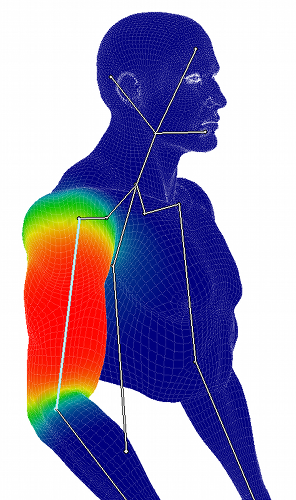
\includegraphics[scale=0.35]{skel.png}
\caption{Skeletal weighting function for arm's bone (Image obtained from http://rodolphe-vaillant.fr).}
\label{skel}
\end{figure}

As we said before, a point of the shape can be assigned to multiple bones. So, in the ideal case, for each point all its weights (for each bone) have to sum 1. The idea is that each point have to follow the corresponding bones movement. The movement of the skeleton is performed in a hierarchical manner. A rigid local transformation is defined for each bone and the global one is computed applying this transformation after parent's transformation. 

The idea is to update the position of each point of the shape performing all the required transformations to allow the bone following. So, first we have to take the point from the world space to the bone space (which has the origin in the parent's joint) and then apply the corresponding accumulated transformation. For a point $p$, the new point $p'$ is given by:
\[
	p' = \sum w_k T_k(t) B_k^{-1} p
\]

where $k$ corresponds to the bone index, $w_k$ is the bone weight, $t$ is the time which defines the current pose of the animation, $T_k(t)$ is the bone's transform in the world space (accumulated transform) and $B_k^{-1}$ is the inverse of the bone to world transform ($B_k$).

This technique produces some artifacts in the resultant shape, volume is not well preserved. Other techniques address these problems without decreasing too much the performance. For example, the dual quaternion deformation \cite{dual} uses a spherical interpolation instead of a linear one, with better performance than other approaches.

\section{Implementation}

We used some classes of Pinocchio \cite{pinocchio} library to manage motion and skeletons. This library was developed for automatic rigging of skeletons but has an animation module which is helpful for us to read and represent data. In this library they use a class Transform to represent a rigid transform matrix using quaternions. The following code is used to compute the transforms for each bone in the world space. "$Transform<>(-match[prevV])$" is the $B_k^{-1}$ transform matrix, "$ts[i]$" is the local transform in the bone space and "$tm[prevV]$" is the corresponding transform of the parent's bone. So, the order matters. The skeleton is ordered following a hierarchical scheme. For example, typically the root of a human skeleton is located in the back. It is important to say that "$ts[i]$" is computed for a given time based on the input motion.

\begin{lstlisting}[basicstyle=\footnotesize\ttfamily ,breaklines=true, frame=single]
for (i = 0; i < (int)ts.size(); ++i) 
{
	int prevV = origSkel.fPrev()[i + 1];
	out.push_back(Transform<>(tm[prevV]) * ts[i] * Transform<>(-match[prevV]));
	tm.push_back(out.back() * match[i + 1]);
}
\end{lstlisting}

Then we can update the vertex positions just applying the sum of these weighted transform matrices. If we want to use shaders we can send all of these transforms to the program and as vertex data the corresponding weights. But sending all weights for all bones is unnecessary because a vertex, which can be far from a bone, can have a weight of 0. Instead of sending all weights we can send the most important ones (higher weights). So, for each vertex we can send, for example, three weights and the corresponding bone indices. In the following code we present a vertex shader where  $boneIDs$ and $boneWeights$ encode the bone indices and the bone weights respectively. We also have a uniform containing all transform matrices (for each bone) for the current time. Then we have to compute the sum of the corresponding transforms and apply it to the vertex position. Due that in our shader we use normal, tangent and bitangent vectors, we have to compute the new vectors applying the transforms.

\begin{lstlisting}[basicstyle=\footnotesize\ttfamily ,breaklines=true, frame=single]
#version 430

in layout(location=0) vec3 position;
in layout(location=1) vec3 vertexColor;
in layout(location=2) vec3 vertexNormal;
in layout(location=3) vec2 texCoord2D;
in layout(location=4) vec3 vertexTangent;
in layout(location=5) vec3 vertexBitangent;
in layout(location=6) vec3 boneIDs;
in layout(location=7) vec3 boneWeights;

const int NR_BONES = 17;

uniform mat4 modelToProjectionMatrix;
uniform mat4 modelToWorldMatrix;
uniform vec3 aditionalProperties;
uniform mat4 mBones[NR_BONES];

out vec3 normalWorld;
out vec3 vertexPositionWorld;
out vec3 theColor;
out vec2 texCoord;
out vec3 tangentWorld;
out vec3 bitangentWorld;

void main()
{
	mat4 BoneTransform = mBones[int(boneIDs[0])] * boneWeights[0];
    BoneTransform += mBones[int(boneIDs[1])] * boneWeights[1];
    BoneTransform += mBones[int(boneIDs[2])] * boneWeights[2];
	
	vec4 animationPos = BoneTransform * vec4(position, 1.0);
	vec4 animationNormal = BoneTransform * vec4(vertexNormal, 0);
	vec4 animationTangent = BoneTransform * vec4(vertexTangent, 0);
	vec4 animationBitangent = BoneTransform * vec4(vertexBitangent, 0);
	
	gl_Position = modelToProjectionMatrix * animationPos;
	normalWorld = normalize(vec3(modelToWorldMatrix * animationNormal));
	tangentWorld = vec3(modelToWorldMatrix * animationTangent);
	bitangentWorld = vec3(modelToWorldMatrix * animationBitangent);
	vertexPositionWorld = vec3(modelToWorldMatrix * animationPos);
	theColor = vertexColor;
	float ps = aditionalProperties[0];
	gl_PointSize = ps;
	//gl_PointSize = 10.f;
	texCoord = texCoord2D;
}
\end{lstlisting}

\section{Conclusion}
The Skeletal Subspace Deformation (SSD) is not a robust technique and presents some artifacts which have an important impact in the final animation. There exist better techniques which are better than SSD and maintain a good performance.
The implementation presented here works when the skeleton has a few number of bones. When this number is too large it can produce a bottle neck in the transform computation or when sending the uniforms to the shader program.

\bibliographystyle{alpha}
\bibliography{main}

\end{document}
